\documentclass[a4paper,10pt]{article}
\usepackage[utf8]{inputenc}
\usepackage{amssymb}
\usepackage{amsmath}
\usepackage{fullpage}
\usepackage{hyperref}
\usepackage{graphicx}
\usepackage{listings}
\usepackage{color}

\definecolor{mygreen}{rgb}{0,0.6,0}
\definecolor{mygray}{rgb}{0.5,0.5,0.5}
\definecolor{mymauve}{rgb}{0.58,0,0.82}

\lstset{ 
  backgroundcolor=\color{white},   % choose the background color; you must add \usepackage{color} or \usepackage{xcolor}; should come as last argument
  basicstyle=\footnotesize,        % the size of the fonts that are used for the code
  breakatwhitespace=false,         % sets if automatic breaks should only happen at whitespace
  breaklines=true,                 % sets automatic line breaking
  captionpos=b,                    % sets the caption-position to bottom
  commentstyle=\color{mygreen},    % comment style
  deletekeywords={...},            % if you want to delete keywords from the given language
  escapeinside={\%*}{*)},          % if you want to add LaTeX within your code
  extendedchars=true,              % lets you use non-ASCII characters; for 8-bits encodings only, does not work with UTF-8
  firstnumber=1,                   % start line enumeration with line 1000
  frame=single,	                   % adds a frame around the code
  keepspaces=true,                 % keeps spaces in text, useful for keeping indentation of code (possibly needs columns=flexible)
  keywordstyle=\color{blue},       % keyword style
  language=Python,                 % the language of the code
  morekeywords={*,...},            % if you want to add more keywords to the set
  numbers=left,                    % where to put the line-numbers; possible values are (none, left, right)
  numbersep=5pt,                   % how far the line-numbers are from the code
  numberstyle=\tiny\color{mygray}, % the style that is used for the line-numbers
  rulecolor=\color{black},         % if not set, the frame-color may be changed on line-breaks within not-black text (e.g. comments (green here))
  showspaces=false,                % show spaces everywhere adding particular underscores; it overrides 'showstringspaces'
  showstringspaces=false,          % underline spaces within strings only
  showtabs=false,                  % show tabs within strings adding particular underscores
  stepnumber=1,                    % the step between two line-numbers. If it's 1, each line will be numbered
  stringstyle=\color{mymauve},     % string literal style
  tabsize=4,	                   % sets default tabsize to 2 spaces
  title=\lstname                   % show the filename of files included with \lstinputlisting; also try caption instead of title
}



\title{\vspace{-2cm}NUR - Assignment 2 }
\author{Amy Louca (1687077)}

\begin{document}

\maketitle

\begin{abstract}
This solution paper is part of the course 'Numerical Recipes in Astrophysics'. The code introduction section will explain briefly some additional details on the code that are not shown/explained in the other sections and how the general code lay-out of each question looks like. Section one will discuss the random number generator that has been used throughout the paper and the goodness of it. Section 2 will use this RNG for the creation of a Gaussian random field with the use of inverse fourier transforms. Afterwards, the linear growth factor that is introduced in cosmology is found as a function of time with the use of a numerical ODE solver. Section 4 explains how a simulation can be made of the initial conditions of the Universe, following with section 5 which looks in more detail in mass assignment schemes. With the use of logistic regression, $\gamma$-ray burst are classified in section 6. Then finally a Barnes-Hut quadtree is build for 1200 particles, where the masses and positions were given.
\end{abstract}

\section*{Code Introduction}

The complete code of this solution paper works as follows. Each question has its own python file that includes all the sub-questions. Whenever some functions need to be shared between (sub-)questions, they are added to the general 'functions' python file. These shared functions are then shown at the beginning of every main-question. The instances and imports that were used in this class are shown below.

\lstinputlisting[firstline = 1, lastline = 30]{functions.py}
\newpage
The python file of each main question has a special lay-out that holds for all questions. Each main question python file contains a class that contains all subquestions and some extra functions needed for some subquestions. These extra functions are put in this class and not in functions.py because they were only used for one subquestion. The code that runs these programs is not shown in each question. Therefore, a demo is shown below,

\lstinputlisting[firstline = 7,lastline = 17]{Q1.py}
Then at the end of each program, the classes are called by,

\lstinputlisting[firstline = 307,lastline = 308]{Q1.py}


\section{Normally distributed pseudo-random numbers}
A normally distributed pseudo-random number generator can be split into two parts. To start with, a uniform pseudo-random number generator is needed. The uniform distribution can then be transformed to a normal distribution given a mean, $\mu$, and variance, $\sigma^2$. The Kolmogorov-Smirnov test and Kuiper's test can then be executed to test how consistent the pseudo random distribution is with a normal distribution. The code that is shared in this section is given below.

\lstinputlisting[firstline = 32,lastline = 204]{functions.py}


\subsection{Uniform distributed pseudo-random numbers}
The uniform distribution used in this solution paper is obtained with the use of the so-called 'multiply with carry' and the XOR-shift method. The multiply with carry method makes use of the function:
\begin{equation}
x_{\mathrm{new}} = a\cdot(x_{old}\& [2^{32} - 1]) + (x_\mathrm{old} >> 32)
\end{equation}
Here $a$ is a constant value that is set to $a  = 4294957665$, $x_{\mathrm{old}}$ is an integer between $0 < x < 2^{64}-1$. The ampersand sign is a bitwise AND operator and the $>>$ sign is a shift operator, where the bits of an integer are shifted to the right 32 times. How the PRNG in this exercise works is as follows. First the seed is updated with the use of the XOR-generator. The output of the XOR-generator is converted to an unsigned 64-bit integer, to make sure that the seed always has 64 bits. This newly updated seed is subsequently given to the MWC function. Only the smallest 32 bits are taken from the output. The final outcome is then divided by the maximum integer that the MWC can possibly output, which is $2^{32} - 1$ (since only the smallest 32 bits are used from the MWC).
The code used to create the uniform distribution is given below. 
The output of the code are 3 different plots. The first plot is random number $x_i$ scatter plotted against random number $x_{i+1}$, where $i$ is $i = 0,1,2,...., 999$ (i.e. in total there are 1000 random numbers created ). The second plot is the pseudo random value $x_i$ plotted against the iterations, $i$, also for 1000 random numbers. The final plot is a histogram of one million pseudo random numbers.

\lstinputlisting[firstline=19,lastline=47]{Q1.py}


\begin{figure}[h]
\vspace{-2.2em}
\centering
\includegraphics[scale=0.4]{plots/rand_nums.png}
\end{figure}

\begin{figure}[h]
\centering
\includegraphics[scale=0.45]{plots/unif_dist.png}
\caption{Upper left: scatter plot of random value $x_i$ against random value $x_{i+1}$, upper right:  random value plotted against iteration $i$, bottom: histogram of one million pseudo random numbers.}
\end{figure}
The first scatter plot seems to be quite uniformly distributed for 1000 gaussian random numbers. At some points it can be seen that there are some gaps, however these remain relatively small. The right plot of figure 1 shows how the value of the random number changes over every iteration. If the generated values come completely from a pseudo random number generator, one expects this plot to look similar like a white noise vs. time plot. \footnote{This comparison is made because the plot reminded me of white noise.} With an exception of a few gaps (e.g. see gap around iteration 500) the generated values do indeed seem to create such white noise. Finally, when looking at the histogram which is created from one million generated pseudo random numbers, it again seems to be extremely uniform. It is expected that for 20 bins, each bin fluctuates around the 50000, with a $1\sigma$ of $\sqrt{50000}$. The biggest fluctuation that was found was of the order $\sim 450$, which is, unfortunately roughly double the $1\sigma$ value. However, this deviation still remains small and therefore the PRNG is not adjusted any further for this solution paper.

\subsection{Box-Muller transformation}
Transforming a uniform distribution to a normal distribution can be done with the use of the Box-Muller transform. The Box-Muller transform goes as follows. Suppose we want two independent ($\mathcal{P}(x,y) = \mathcal{P}(x)\mathcal{P}(y)$) variables that are both drawn from gaussian distributions:
\begin{gather*}
X \sim G(\mu,\sigma^2) = \frac{1}{\sqrt{2\pi\sigma^2}}\exp\left(-\frac{1}{2}\left[\frac{x-\mu}{\sigma}\right]^2\right)\\
Y \sim G(\mu,\sigma^2) = \frac{1}{\sqrt{2\pi\sigma^2}}\exp\left(-\frac{1}{2}\left[\frac{y-\mu}{\sigma}\right]^2\right)\
\end{gather*}
The joint distribution of these independent variables then becomes:
\begin{equation*}
\mathcal{P}(x,y) = \frac{1}{2\pi\sigma^2}\exp\left(-\frac{1}{2}\left[\frac{x-\mu}{\sigma}\right]^2\right)\exp\left(-\frac{1}{2}\left[\frac{y-\mu}{\sigma}\right]^2\right) = \frac{1}{2\pi\sigma^2}\exp\left(-\frac{1}{2\sigma^2}\left[(x-\mu)^2 + (y-\mu)^2\right]\right)
\end{equation*}
This equation can be converted to polar coordinates. Namely, take $x-\mu = r\sin(\theta)$, and $y - \mu = r\cos(\theta)$. Then the above equation reduces to:
\begin{equation*}
\mathcal{P}(x,y) = \mathcal{P}(r,\theta) = \frac{1}{2\pi\sigma^2}\exp\left(-\frac{r^2}{2\sigma^2}\right)
\end{equation*}

It can be seen from figure \ref{joint_dist} that the shape of the joint distribution of the two gaussians resembles a disk. The polar coordinates $r$ and $\theta$ can now be seen as the distance from one scatter point to the centre (=mean) of the circle and as the angle between the scatter point and the x-axis (or y-axis). Therefore, $\theta$ falls within $0 \leq \theta \leq 2\pi$. Since the angle of every scatter point is uniformly scattered (i.e there are as many scatter points on, for example, $\theta = 0$ as $\theta = \pi$), $\theta$ can be written in terms of a uniform distribution: $\theta = 2\pi \mathrm{U}(0,1)$.

\begin{figure}[h]
\centering
\includegraphics[scale=0.5]{joint_dist.png}
\caption{A scatter plot of the joint distribution of variables from two gaussians with mean $\mu = 3$, and standard deviation $\sigma = 2.4$. The red circles have $1\sigma$, $2\sigma$, and $3\sigma$ radii (small circle to big circle respectively) and are centered around the means. }
\label{joint_dist}
\end{figure}
Marginalizing the $\theta$ term out by integrating over the joint distribution gives:
\begin{equation*}
\mathcal{P}(r) = \int_0^{2\pi} \frac{1}{2\pi\sigma^2}\exp\left(-\frac{r^2}{2\sigma^2}\right) \mathrm{d}\theta = \frac{1}{\sigma^2} \exp\left(-\frac{r^2}{2\sigma^2}\right)
\end{equation*}

Now calculating  and working out the cumulative distribution for a random radius $R$,
\begin{gather*}
\mathcal{P}(r \leq R) = \int_0^R \frac{1}{\sigma^2} \exp\left(-\frac{r^2}{2\sigma^2}\right) r\mathrm{d}r = \frac{1}{\sigma^2}\left[-\sigma^2 \exp\left(-\frac{r^2}{2\sigma^2}\right)\right]_0^R\\
= 1- \exp\left(-\frac{R^2}{2\sigma^2}\right)
\end{gather*}
Note that the factor $r$ appears in the integral because we are dealing with polar coordinates.  Radius $R$ can be any number between $0$ and $\infty$. If $R = \infty$ then $\mathcal{P}(r \leq \infty) = 1 - exp\left(\infty\right) = 1$, and if $R = 0$ then $\mathcal{P}(r \leq 0) = 1 - exp\left(0\right) = 0$. Therefore, the term $1 -  \exp\left(-\frac{R^2}{2\sigma^2}\right)$ falls within $0 \leq < \mathcal{P}(r \leq R) \leq 1$, and thus,
\begin{equation*}
1 -  \exp\left(-\frac{R^2}{2\sigma^2}\right) = 1 - \mathrm{U}(0,1)
\end{equation*}
Note that $R$ can be any value between zero and infinity and therefore it is also possible to write the equation above in terms of $r$. Solving this gives,
\begin{equation*}
\exp\left(-\frac{r^2}{2\sigma^2}\right) = \mathrm{U}(0,1)\\
r = \sqrt{-2\sigma^2\ln\left( \mathrm{U}(0,1)\right)}
\end{equation*}
Substituting $r$ and $\theta$ back into the expressions $x-\mu = r\sin(\theta)$ and $y - \mu = r\cos(\theta)$ gives:
\begin{gather}
x = \sqrt{-2\sigma^2\ln\left( \mathrm{U}(0,1)\right)}\sin(2\pi\mathrm{U}(0,1)) + \mu \\
y = \sqrt{-2\sigma^2\ln\left( \mathrm{U}(0,1)\right)}\cos(2\pi\mathrm{U}(0,1)) + \mu
\end{gather}
where $\mathrm{U}(0,1)$ is a random variable drawn from the uniform distribution. Note that the variable drawn from the uniform distribution in the natural logarithm is not the same as the variable drawn from the uniform distribution in the sin/cos terms. 
The expressions above are also known as the Box-Muller transforms.
The code used to work out question 1b is shown below\footnote{note that the box-muller transform itself is not in this python file, because it is a shared function in this exercise and is therefore listed in the introduction of Q1.},


\lstinputlisting[firstline = 49, lastline = 78]{Q1.py}

The output of the code is a histogram of 1000 variables drawn from a normal distribution with $\mu = 3$ and $\sigma = 2.4$.
\begin{figure}[h]
\centering
\includegraphics[scale=0.55]{plots/normal_dist.png}
\vspace{-1.5em}
\caption{Probability histogram of 1000 variables drawn from a normal distribution with $\mu = 3$ and $\sigma = 2.4$, with 14 bins. The green line represents the actual gaussian distribution with  $\mu = 3$ and $\sigma = 2.4$, and the black striped lines represent the $\sigma$ lines, where each line is indicated which sigma line it represents in the plot.}
\end{figure}

The figure shows quite some resembles between the histogram and the actual gaussian, which indicates that the drawn variables most probably do follow the gaussian distribution with $\mu = 3$ and $\sigma = 2.4$. The next section tests if this is actually the case.
\newpage
\subsection{KS-test}
A Kolmogorov-Smirnov test (KS-test) can be used to test whether the RNG is able to produce a normal distribution with the use of the Box-Muller transform. The KS-test approximates the cumulative distribution of the drawn variables and compares it with the actual cumulative distribution of the probability distribution that one wants to compare it with. Given a set of variables drawn randomly from a distribution, the approximated CDF of variable $x_i$ can be found by counting how many variables have a lower value than $x_i$. This can be efficiently done by first sorting the randomly drawn variables. The sorting is done with the quicksort algorithm as shown in the code. The approximated CDF then becomes:
\begin{equation*}
S_N(x_i)= \frac{k+1}{N}
\end{equation*}
where $N$ is the total number of variables and $k$ is the number of variables that have a lower value than $x_i$. The actual CDF could be calculated with the use of a numerical integration method. However, this will take an enormous amount of time to compute. Therefore, a numerical approximated version of the CDF is used in this question. The CDF of a  normal distribution s given by:
\begin{equation*}
\mathcal{P}(x \leq X) = \frac{1}{2}\left[1 + \mathrm{erf}\left(\frac{X-\mu}{\sigma \sqrt{2}}\right)\right]
\end{equation*}
Where $\mathrm{erf}$ is the error function which is simply the integral of sigmoid shape: $\mathrm{erf}(x) = \frac{1}{\sqrt{\pi}}\int_{-x}^x e^{-(x')^2}\mathrm{d}x'$. For a standard normal distribution the equation shown above reduces to,
\begin{equation*}
\mathcal{P}(x \leq X) = \frac{1}{2}\left[1+\mathrm{erf}\left(\frac{X}{\sqrt{2}}\right)\right]
\end{equation*}
According to Abramowitz and Stegun\footnote{https://en.wikipedia.org/wiki/Error\_function\#Numerical\_approximations}, the error function can be approximated by,
\begin{equation*}
\mathrm{erf}(x) \approx 1 - (a_1 t + a_2 t^2 + a_3t^3 + a_4t^4 + a_5t^5)e^{-x^2}
\end{equation*}
where $t = \frac{1}{1+px}$, and $p = 0.3275911$, $a_1 = 0.254829592$, $a_2 = -0.284496736$, $a_3 = 1.421413741$, $a_4 = -1.453152027$, adn $a_5 = 1.061405429$. If used correctly, this approximation has a maximum error of $1.5\cdot 10^{-7}$.
Having found the approximated CDF of the actual distribution $\mathcal{P}(x\leq X)$, and the approximated CDF of the drawn variables $S_N(x_i)$, the K-S statistic is given by,
\begin{equation*}
D = \underset{-\infty \leq x \leq \infty}{\max}|S_N(x_i) - \mathcal{P}(x \leq x_i)|
\end{equation*}
where $x_i$ is the value of the drawn variable. One should take into account that the cdf of a discrete distribution is a step function and therefore the previous value of the discrete cdf should always be taken into account in determining the distance between the actual CDF and the discrete CDF. The p-value of the observed KS-statistic is then given by:
\begin{equation*}
\mathcal{P}(D > \mathrm{observed}) = Q_{KS}\left(\left[\sqrt{N} + 0.12 + \frac{0.11}{\sqrt{N}}\right]D\right) = Q_{KS}(z)
\end{equation*}
where $N$ is the number of variables that were drawn,\footnote{This only holds for a discrete distribution that is compared with a continuous distribution.} and $Q_{KS}$ is given by:
\begin{equation*}
Q_{KS}(z) = \frac{\sqrt{2\pi}}{z}\sum_{k=1}^{\infty} e^{-(2k-1)^2\pi^2/(8z^2)}
\end{equation*}
This can be approximated as,
\begin{equation}
Q_{KS}(z) \approx \begin{cases}
1 - \frac{\sqrt{2\pi}}{z}\left[(e^{-\pi^2/(8z^2)}) + (e^{-\pi^2/(8z^2)})^9 + (e^{-\pi^2/(8z^2)})^{25}\right] \mathrm{\ \ \ (z < 1.18)}\\
2\left[(e^{-2z^2}) - (e^{-2z^2})^4 + (e^{-2z^2})^9\right] \mathrm{\ \ \ \ \ \ \ \ \ \ \ \ \ \ \ \ \ \ \ \ (z\geq 1.18)}
\end{cases}
\end{equation}
The code used for the Kolmogorov-Smirnov test is shown below,

\lstinputlisting[firstline = 80, lastline = 146]{Q1.py}

The output of the code is a graph of the p-values from the KS-test for different amount of samples drawn from the standard normal distribution that has been generated with the RNG described in the previous section. These p-values are also compared with the p-values produced by a scipy package that computes the KS-test.

\begin{figure}[h]
\centering
\includegraphics[scale=0.5]{plots/KS-test.png}
\caption{Graph of the KS-test where the vertical axis represents the p-value, and the horizontal axis the amount of samples that are drawn from the standard normal distribution, in log-space. The red line is the own-written KS-test , the blue line is the KS-test as produced by the scipy package, and the green dotted horizontal line is the line that represents a p-value of 0.05.}


\label{KS-test}
\end{figure}

It can be seen from figure \ref{KS-test} that the p-values of the samples drawn from the standard normal distribution all lie above $p=0.05$ for large sample sizes\footnote{The 'p-value' can be seen as the probability to reject to null hypothesis, which is in this case: NULL: the generated samples are drawn from a standard normal distribution}. On top of that, both the scipy package and the own implementation seem to produce quite similar results. The latter point indicates that the own implementation has been done correctly. The distribution in figure \ref{KS-test} fluctuates quite a bit. An explanation for this could be that the samples drawn from the distribution are not completely random but rather pseudo random. 

The fact that all p-values are above the 0.05 line is a strong indication that the variables drawn from the RNG that are transformed with the Box-Muller method, follow the standard normal distribution.

\subsection{Kuiper's test}

Another, perhaps even better, test that can be used to evaluate the goodness of the RNG, is the Kuiper's test. This test is very similar to the KS-test, though it uses a different statistic and has a different cumulative distribution for the p-values. The method is the same, and therefore the approximations for the actual CDF of a standard normal distribution and the CDF of the samples are done in the same way as discussed in the previous section. 
The Kuiper's statistic is given by,
\begin{equation*}
V = D_{+} + D_{-} =  \underset{-\infty \leq x \leq \infty}{\max} [S_N(x_i) - \mathcal{P}(x \leq x_i)] +  \underset{-\infty \leq x \leq \infty}{\max} [\mathcal{P}(x \leq x_i) - S_N(x_i)]
\end{equation*}
So instead of looking at the absolute distance between the two distributions at one value, it takes the sum of the maximum distance of $S_N(x_i)$ above and below $\mathcal{P}(x \leq x_i)$. The p-value is then given by,
\begin{equation*}
\mathcal{P}(V > \mathrm{observed}) = Q_{KP}([\sqrt{N}+0.155+\frac{0.24}{\sqrt{N}}]V) = Q_{KP}(\lambda)
\end{equation*}
Here $N$ is the number of samples and $Q_{KP}$ is given by,
\begin{equation*}
Q_{KP}(\lambda) = 2\sum_{j=1}^{\infty} (4j^2\lambda^2 -1 )e^{-2j^2\lambda^2}
\end{equation*}

This equation is not approximated in the code. Instead of summing over all the values, a while-loop is implemented and is only stopped if the absolute of the previous $Q_{KP}$ value minus the current $Q_{KP}$ value is smaller than $1\cdot10^{-8}$. The code that is used to calculate the Kuiper's test is shown below.
\lstinputlisting[firstline = 148, lastline = 234]{Q1.py}

The output of the code is a similar plot as shown in the previous section, but now done with the Kuiper's test (i.e. a graph of the p-values for different sample sizes and for both the own implementation and the astropy implementation).
\begin{figure}[h]
\centering
\includegraphics[scale=0.5]{plots/kuiper-test.png}
\caption{Graph of the Kuiper's test where the vertical axis represents the p-value, and the horizontal axis the amount of samples that are drawn from the standard normal distribution, in log-space. The red line is the own-written KS-test , the blue line is the Kuiper's test as produced by the astropy package, and the green dotted horizontal line is the line that represents a p-value of 0.05.}
\label{kuiper}
\end{figure}

Figure \ref{kuiper} shows that almost all computed p-values seem to be equal to or greater than 0.05. However, the p-values obtained from the own implementation of the first few sample sizes do not match quite as good with the astropy version as it did before with the KS-test with the scipy version. One explanation could be that the calculations for $Q_{KP}$ are done differently in astropy. Nevertheless, the p-values do seem to match quite well for larger sample sizes, which is of course the most important part. The fact that two p-values lie below the 0.05 line is not dramatic, since these are relatively small sample sizes. If this would happen at the largest sample size then one would have to question whether the NULL hypothesis is correct or not. All in all, both the kuiper's test and the KS-test show that the samples drawn from the distribution match the standard normal distribution quite well for large sample sizes. 


\subsection{Testing various given distributions}

Now that it has been shown that the PRNG can create a standard normal distribution quite well, it can also be tested on other distributions. Given an unknown distribution, one can test whether it follows a standard normal distribution by comparing the samples with some samples of the standard normal distribution created by the PRNG described above. In this section, 10 unknown distributions are compared with a distribution created from the own implementation. This is done with the use of the KS-test again, though now some slight adjustments have been made to the KS-test. The KS-test described in section 1.3 is for a discrete distribution that is being compared with a continuous distribution. For this question we now instead have two discrete distributions. How this is done is as follows. To start with, the samples from both discrete distributions are sorted, with the use of the quicksort algorithm again. The KS-statistic is then determined by counting both distributions again, but now in a special way. When looking at the sorted sample values, if the second sample value of distribution 1 is greater than the second sample value of distribution 2, it means that distribution 2 has increased in step size at an earlier point. This means that the distance between the CDF distribution 1 and distribution 2 is determined by counting how much higher one distribution is at a certain point than the other. With the use of this logic, the distances of the CDF of both functions can be determined by comparing their sample values. When the sample value of one distribution at a certain point is lower than the other, then the step size is increased. When having found the maximum distance, the p-value can be calculated. This is done in the similar way as described in section 1.3. The only difference here is that the value of the total number of samples $N$ is approximated differently. Given that the first distribution has $N_1$ samples and the second distribution has $N_2$ samples, the effective number of samples is,
\begin{equation*}
N_e  = \frac{N_1 N_2}{N_1 + N_2}
\end{equation*}
In this question the amount of samples for both distributions is the same and therefore $N_e = 0.5N$, with $N$ is the number of samples used for both distributions. So the value $z$ (see section 1.3) is now given by $z = \left(\sqrt{N_e} + 0.12 + \frac{0.11}{\sqrt{N_e}}\right)D$, where $D$ is the KS-statistic.\\
Each unknown distribution is compared with the distribution created from the PRNG and the box-muller transformation, for $\mu =0$ and $\sigma = 1$. The code that has been used for this comparison is shown below,
\lstinputlisting[firstline = 236, lastline = 305]{Q1.py}
\vspace{-1em}
The output of the code is 10 individual plots that, one for each column of samples. Each plot contains the p-values for different sample sizes. The plots also contain the horizontal line at $p = 0.05$, which simply indicates the p-value of 0.05. If the calculated p-value falls below this line, then the null hypothesis is rejected. In this case, the null hypothesis is: the unknown distribution is sampled for a standard normal distribution. One assumption that has to be made here is that the distribution which it is being compared to (my own distribution) is sampled from a standard normal distribution. This assumption is quite fair since it has been shown previously that this is most probably the case.
It can be seen from the plots that quite a lot of distributions have small p-values for large sample sizes. This means that also quite a lot of distributions are not similar to my own standard normal distribution. The p-values for the first three plots (column 0 to 2) are quite high for low sample sizes and extremely low for high sample sizes. The reason that we can reject the null hypothesis for these plots is that large sample sizes are more statistical relevant then small sample sizes. For example, it could be that the first 10 samples of these columns seemed to be distributed as a standard normal distribution, however 10 samples don't say much. For the high sample sizes we can definitely say that they don't match with our own standard normal distribution. The third column  (plot 4) shows something differently. The p-value for this distribution fluctuates for small sample sizes around the p=0.05 line and the for the large sample sizes it increases a lot. This gives us an indication that this distribution is most probably a standard normal distribution. The plot of the fifth distribution resembles the first 3 distributions a lot and can therefore also be rejected as being a standard normal distribution. Then we have the sixth distribution which is quite an interesting one. This one fluctuates quite a lot for different sample sizes. Only for a few sample sizes the p-value is below the 0.05. Nonetheless, for the largest sample sizes this should not happen if it was actually a standard normal distribution. With a bit of doubt, this distribution is therefore rejected to be a standard normal distribution as well. Then for the last 4 distributions we see similar shapes as for the first three again. The distributions seem to follow a standard normal distribution for small sample sizes, but when the number of samples increases it becomes quite clear that this is not actually the case. Therefore the null hypothesis is rejected for these distributions as well. The only distribution that can be said to be standard normal, with certainty, is the fourth distribution.

\begin{figure}[h]
\vspace{-1.3em}
\centering
\includegraphics[scale=0.5]{plots/KS-test_column_1.png}
\end{figure}

\vspace{-2.6em}

\begin{figure}[h]
\centering
\includegraphics[scale=0.5]{plots/KS-test_column_3.png}
\end{figure}
\begin{figure}[h]
\vspace{-1cm}
\centering
\includegraphics[scale=0.5]{plots/KS-test_column_5.png}
\end{figure}
\begin{figure}[h]
\centering
\includegraphics[scale=0.5]{plots/KS-test_column_7.png}
\end{figure}
\begin{figure}[h]
\centering
\includegraphics[scale=0.5]{plots/KS-test_column_9.png}
\caption{10 p-value vs. number of sample plots for 10 different unknown distributions. Each plot indicates which column is being compared with my own distribution. The p-values of 0.05 are indicated by the green dotted lines.}
\end{figure}

\clearpage


\section{Making an initial density field}

The density field of a cosmological simulation can be made with the use of the previously made pseudo random number generator. A Gaussian random field is made in Fourier space. The dispersion of the gaussian field is given by,

\begin{equation*}
\sigma^2 = P(k) \sim k^n
\end{equation*}
For this exercise it is assumed that the normalization constant is equal to 1 such that $\sigma^2 = k^n$. The fourier space matrix that is constructed consists of complex entries that are drawn from the gaussian distribution with mean zero, $\mu = 0$, and variance equal to the dispersion, $\sigma^2 = k^n$. Here $k$ are the wavenumbers and $n$ determines how steep the power spectrum will be in loglog space. The matrix that is constructed has a special symmetry, namely $\bar{Y}(-\textbf{k}) = \bar{Y}^*(\textbf{k})$ (i.e. the elements in the fourier- matrix are symmetric). This symmetry has to hold such that the inverse fourier transform generates real numbers, instead of complex numbers. The symmetry is obtained in the following way. If $M_{k_x,k_y}$ are the randomly created complex values in the matrix, with $k_x$ and $k_y$ being the wavevectors containing the wavenumbers, then the following symmetries should hold: $M_{k_x,k_y} = M_{-k_x,-k_y}^*$. However, if $k_x = 0$ and $k_y = 0$ then we assign the value $0 + 0i$ to this matrix element. This is because of the power $n$. If this power is negative then this matrix element will go to infinity for $k_x,k_y = 0$. Then we also have to take care of the so-called nyquist frequency $k_{\mathrm{nyq}}$. The nyquist frequency element does not have a corresponding negative wavenumber. Therefore the only way to have a complex value that equals its non-negative conjugate, it to assign only a real-value to this matrix element. Therefore, $k_x = k_y = k_{\mathrm{nyq}} = \mathbb{R}$. Another property of the nyquist frequency is $k_{\mathrm{nyq}} = -k_{\mathrm{nyq}}$. This ensures that if either $k_x = k_{\mathrm{nyq}}$ or $k_y = k_{\mathrm{nyq}}$, the matrix elements do have a complex conjugate value. The only exception in this particular row and column is whenever $k_x = 0$ and $k_y = k_{\mathrm{nyq}}$ (or the other way around), then we have the same problem as when having two nyquist frequencies again. Therefore, these matrix elements have to be real-valued as well. When the symmetric matrix has been created, the inverse fourier transform is calculated with the use of a scipy package. This package normalizes the inverse fourier transform by dividing it by the number of gridpoints $N$ (in 2d). For this exercise a minimal physical size has also been set. The wave-vector $\textbf{k}$ is affected by this minimal physical size, because all its elements are divided by the maximal physical size. If the minimal physical size is $s_{\mathrm{min}}$, then the maximal physical size is $s_{\mathrm{max}} = s_{\mathrm{min}}\cdot N$, where $N$ is the number of gridpoints. So in the cases above the maximum physical size is 1024 Mpc, since there are 1024 gridpoints and the minimal physical size is set to 1 Mpc. The wavenumbers are given by $k = \frac{2\pi}{\lambda}$, where $\lambda$ is a physical size of an object. So for a wave-vector with entries $k = 0, \pm 1, \pm 2, ... \frac{N}{2}$, we get as minimum wavenumber $k_{\mathrm{min}} = 1\cdot\frac{2\pi}{s_{\mathrm{max}}}$, with $s_{\mathrm{max}}$ being the maximum physical size. Then for the maximum wavenumber we get $k_{\mathrm{max}} = \frac{N}{2}\cdot \frac{2\pi}{s_{\mathrm{max}}} = \frac{N\pi}{s_{\mathrm{max}}} = \frac{N\pi}{s_{\mathrm{min}}N} = \frac{\pi}{s_{\mathrm{min}}}$.
The code that is used to produce such a matrix that has the correct fourier-symmetry and wavenumbers is given below\footnote{Note that the RNG is also used in this exercise but is not shown here since it has already been shown.},

\lstinputlisting{Q2.py}

The output of the code are three plots for different values of $n$ ($n = -1$, $n = -2$, and $n = -3$). Each plot is created with the exact same random numbers generated by the PRNG described in the previous section. The plots are the inverse fourier transform of the symmetric gaussian filled matrix, which create an initial density field that is gaussian randomly distributed. 

\begin{figure}[h]
\vspace{-1.2em}
\centering
\includegraphics[scale=0.6]{plots/density_field_1.png}
\vspace{-1.5em}
\caption{Gaussian random field for $n = -3$.}
\label{n_3}
\end{figure} 
\begin{figure}[h]
\vspace{-2.5em}
\centering
\includegraphics[scale=0.6]{plots/density_field_2.png}
\vspace{-1em}
\caption{Gaussian random field for $n = -2$.}
\end{figure} 
\begin{figure}[h]
\centering
\includegraphics[scale=0.6]{plots/density_field_3.png}
\caption{Gaussian random field for $n = -1$.}
\end{figure} 
Each of the figures are quite different. For all three power spectra ($n=-1$, $n=-2$, $n=-3$), the dispersion of the gaussian field differs. For $n=-3$ this dispersion is biggest since $k$ is always equal to or smaller than 1. This means that we should see a lot of structure for this particular random gaussian field. Taking a look at the figures, this indeed seems to be the case. When the value for $n$ increases, the amount of structure seen in the density field seem to disappear and it becomes more and more a homogeneous field. 


\section{Linear Structure Growth}

The evolution of density perturbations in the initial universe evolves accordingly to,
\begin{equation*}
\frac{\partial^2 \delta}{\partial t^2}  + 2 \frac{\dot{a}}{a}\frac{\partial \delta}{\partial t} = \frac{3}{2} \Omega_0 H_0^2 \frac{\partial}{a^3}
\end{equation*}
In the early Universe, the density perturbation can be separated in a spatial part and a temporral part: $\partial = D(t)\triangle(\textbf{x})$. Substituting this into the equation above gives,
\begin{equation*}
\frac{\mathrm{d}^2 D}{\mathrm{d}t^2} + 2\frac{\dot{a}}{a}\frac{\mathrm{d}D}{\mathrm{d}t} = \frac{3}{2}\Omega_0H_0^2\frac{1}{a^3}D
\end{equation*}
Knowing how $a$ evolves over time, this second order ODE can be solved analytically and numerically. First the analytical part is solved to check how the linearized density growth factor evolves over time.\footnote{The reason to show the analytical solution first is because there are various numerical methods to solve this second order ODE. If the analytical solution is known before hand, the numerical method can be chosen accordingly to this solution (the most difficult method is not always necessary, so if we are lucky we can use easy numerical methods.)} The assumption is made that we deal with a matter-dominated Einstein-de Sitter Universe, $\Omega_m = 1$. The scale factor then becomes,
\begin{equation*}
a(t) = \left(\frac{3}{2}H_0 t\right)^{2/3}
\end{equation*}
The time derivative of this scale factor is then,
\begin{equation*}
\frac{\mathrm{d}a(t)}{\mathrm{d}t} = \frac{2}{3}\left(\frac{3}{2}H_0t\right)^{-1/3}\cdot \frac{3}{2} H_0 = H_0 \left(\frac{3}{2}H_0 t\right)^{-1/3}
\end{equation*}
Filling this into the differential equation,
\begin{gather*}
\frac{\mathrm{d}^2D}{\mathrm{d}t^2} + 2 \frac{ H_0 \left(\frac{3}{2}H_0 t\right)^{-1/3}}{ \left(\frac{3}{2}H_0 t\right)^{2/3}}\frac{\mathrm{d}D}{\mathrm{d}t} = \frac{3}{2}\Omega_0 H_0^2 \frac{1}{ \left[\left(\frac{3}{2}H_0 t\right)^{2/3}\right]^3} D \\
\frac{\mathrm{d}^2 D}{\mathrm{d}t^2 }+ \frac{2 H_0}{\frac{3}{2}H_0 t}\frac{\mathrm{d}D}{\mathrm{d}t} = \frac{3}{2}\Omega_0 H_0^2 \frac{1}{\left(\frac{3}{2}H_0 t\right)^2} D
\end{gather*}
\begin{equation}
\frac{\mathrm{d}^2D}{\mathrm{d}t^2} + \frac{4}{3t} \frac{\mathrm{d}{D}}{\mathrm{d}t} = \frac{2 \Omega_0}{3 t^2} D
\end{equation}
The general solution to such an equation is given by $D(t) = A\cdot t^{\lambda}$. Substituting this form into the differential equation gives,
\begin{gather*}
\frac{\mathrm{d}^2}{\mathrm{d}t^2}\left(A\cdot t^{\lambda}\right) + \frac{4}{3t} \frac{\mathrm{d}}{\mathrm{d}t}\left(A\cdot t^{\lambda}\right) = \frac{2\Omega_0}{3t^2} A\cdot t^{\lambda}\\
A\lambda(\lambda - 1) t^{\lambda - 2} + \frac{4}{3t}A\lambda t^{\lambda-1} = \frac{2\Omega_0}{3t^2} At^{\lambda}\\
\frac{\lambda(\lambda-1)t^{\lambda}}{t^2} + \frac{4\lambda t^{\lambda}}{3t^2} = \frac{2\Omega_0}{3t^2} t^{\lambda}\\
\lambda(\lambda-1) + \frac{4\lambda}{3} = \frac{2\Omega_0}{3}
\end{gather*}
Recall that $\Omega_0 = \Omega_m = 1$ since we deal with a matter-dominated Universe. Solving this for $\lambda$ gives then,
\begin{gather*}
\lambda^2 + \frac{1}{3}\lambda - \frac{2}{3} = 0\\
\lambda_1  = \frac{2}{3}, \mathrm{\ \ \ \ \ \ } \lambda_2 = -1
\end{gather*}
So the analytical solution for the linearized density growth factor is:
\begin{equation}
D(t) = At^{2/3} + Bt^{-1}
\end{equation}
Where $A$ and $B$ are constants that can be found by filling in the initial conditions. To show how this works, case 1 will be demonstrated. For case 1 we have $D(1) = 3$ and $D'(1) = 2$. The time-derivative of $D$ is $D'(t) = \frac{2A}{3}t^{-1/3} - Bt^{-2}$. Filling in the initial conditions gives: $D(1) = A + B = 3$, $D'(1) = \frac{2A}{3} - B = 2$. Solving this system of equations for $A$ and $B$ gives then: $A = 3$, $B=0$. This can also be done for the other two cases but are not demonstrated here because it's quite straightforward how to solve them. The final equations for the 3 cases are then,
\begin{gather}
\mathrm{Case \ 1: \ \ \ \ \ } D(t) = 3t^{2/3}\\
\mathrm{Case \ 2: \ \ \ \ \ } D(t) = 10t^{-1}\\
\mathrm{Case \ 3: \ \ \ \ \ } D(t) = 3t^{2/3} + 2t^{-1}
\end{gather}
If we fill in $t = 1000$ yr, we get an indication of where the equations converge to. Case 1 is an increasing function that after 1000 yrs becomes $D(1000) = 300$. Case two is a decreasing function that after 1000 yrs becomes $D(1000) = \frac{1}{100}$, and case 3 is also an increasing function where the factor $\frac{2}{t}$ disappears when $t$ increases. This function therefore starts of as case 2 and then at some point switches to case 1. Case 2 is a situation which can easily go wrong if an incorrect numerical solver is used. This is because the values of the density growth get extremely small on larger timescales. Therefore, the Runga-Kutte method is used with an adaptive stepsize control. In particular, the 5th order Runga-Kutta method with adaptive stepsize control is used. The Runga-Kutte method is based on the Euler-method which is one of the easiest methods that can be used to solve first order ODEs.
Since the ODE given in equation 5 is of second order, it might be convenient to first rewrite this equation to two separate first order ODEs. This can be done by making the substitution: $x(t) = \frac{\mathrm{d}D(t)}{\mathrm{d}t}$. Equation 5 can then be written as,
\begin{equation*}
\frac{\mathrm{d}x(t)}{\mathrm{d}t} + \frac{4}{3t}x(t) = \frac{2\Omega_0}{3t^2} D(t)
\end{equation*}
Rewriting this equation gives,
\begin{equation*}
\frac{\mathrm{d}x(t)}{\mathrm{d}t} = -\frac{4}{3t}x(t) + \frac{2\Omega_0}{3t^2} D(t)
\end{equation*}
Using the fact that we deal with a matter-dominated Universe, the final set of ODEs that has to be solved is then,
\begin{gather}
\frac{\mathrm{d}D(t)}{\mathrm{d}t} = x(t)\\
\frac{\mathrm{d}x(t)}{\mathrm{d}t} = -\frac{4}{3t}x(t) + \frac{2}{3t^2} D(t)
\end{gather}
%IETS HIEROVER UITLEGGEN?
By substituting the given initial conditions, the initial conditions for $x(1)$ can be found as well. Since $D'(t) = x(t)$, we simply have that $x(1) = D'(1)$, so the initial conditions for $x$ are simply equal to the initial conditions of the time derivative of $D$ (i.e. $D'(1)$). 
 The code that is used in this exercise is given below.
\lstinputlisting{Q3.py}
The code produces a loglog plot of the numerical and analytical solution to the ODE given above for each case. It can be seen from the below figures (see next page) that the analytical and numerical solutions seem to match extremely well, indicating that the numerical method used in this solution paper is sufficient enough for solving such ODEs.
\begin{figure}[h]
\vspace{-1em}
\centering
\includegraphics[scale=0.5]{plots/ODE_case_1.png}
\end{figure} 

\begin{figure}[h]
\vspace{-1em}
\centering
\includegraphics[scale=0.5]{plots/ODE_case_2.png}
\end{figure}
\begin{figure}[h]
\vspace{-1em}
\centering
\includegraphics[scale=0.5]{plots/ODE_case_3.png}
\caption{The three plots of the numerical (blue) and analytical (red) solutions to the ODE for three different initial conditions. The above image is the case where $D(1) = 3$, $D'(1) = 2$, the middle image is the case where $D(1) = 10$, $D'(1) = -10$, and the last image is the case where $D(1) = 5$, and $D'(1) = 0$.}
\end{figure}

\clearpage
\newpage
\newpage
\section{Zeldovich approximation}
The initial conditions for a cosmological problem can be set up with the use of the so-called Zeldovich approximation. This is a first order linear Lagrangian structure formation model. The simplest form of the approximation is given by,
\begin{equation*}
\textbf{x}(t) = \textbf{q} + D(t)\textbf{S}(\textbf{q})
\end{equation*}

Where $D(t)$ is the linear growth factor that has been shown before in the previous factor.\footnote{Since the expansion factor, $a$, relates to time, $t$, the linear growth factor can also be written as $D(t) = D(a(t))$} The momentum of the particles for the the initial conditions is given by,
\begin{equation*}
\textbf{p} = -(a-\triangle a/2)^2\dot{D}(a-\triangle a/2)\textbf{S}(\textbf{q})
\end{equation*}
Where $a$ is the expansion factor, which relates to the time $t$. The displacement vector $\textbf{S}$ is given by the fast fourier transform, FFT,
\begin{equation*}
\textbf{S}(\textbf{q}) = \alpha \sum_{k_x = - k_{\mathrm{max}}}^{k_{\mathrm{max}}} \sum_{k_y = - k_{\mathrm{max}}}^{k_{\mathrm{max}}}\sum_{k_z = - k_{\mathrm{max}}}^{k_{\mathrm{max}}} i\textbf{k}c_k \exp(i\textbf{k}\cdot\textbf{q})
\end{equation*}
where $\textbf{k}$ is the wave-vector for the $x$, $y$, and $z$ direction, $k_{x,y,z} = \frac{2\pi}{N_g}l,m,n$, with $N_g$ the number of grid points for each direction and $l,m,n = 0,\pm,....,N_g/2$. The power spectrum normalization factor $\alpha$ is normally set to 1, but in this question the the numpy and scipy packages are used to calculate the IFFT above which do need normalization constants. Numpy normalizes a one dimensional IFFT by dividing it by the number of grid points, whereas scipy normalizes a one dimensional IFFT by dividing it by the square root of the number of grid points. Therefore, to obtain the correct $\textbf{S}(\textbf{q})$ one has to multiply the found IFFT by $N_g$ for the numpy package and by $\sqrt{N_g}$ for the scipy package.\footnote{This is for the one dimensional IFFT, for two dimensions the factors would be $N_g^2$ and $N_g$ for numpy and scipy respectively and for three dimensions the factors would be $N_g^3$ and $(N_g)^{3/2}$ for numpy and scipy respectively.} The factor $c_k$ are random numbers given by $c_k = (a_k - ib_k)/2$, with,
\begin{equation*}
a_k = \sqrt{P(k)}\frac{\mathrm{Gauss}(0,1)}{k^2}\neq b_k = \sqrt{P(k)}\frac{\mathrm{Gauss}(0,1)}{k^2}
\end{equation*}
To make sure that the FFT is real, the gaussian random fields should satisfty $c_k$ = $c_{-k}^*$. The next section will discuss in steps how this initial field is obtained. The code that is shared in this section is given below,

\lstinputlisting[firstline = 206, lastline = 287]{functions.py}


\subsection{Linear Growth Factor - integration}

The linear Growth factor as a function of the expansion factor, $a$, is one of the ingredients for finding the initial conditions of the particles. This growth factor in integral form is given by,
\begin{equation*}
D(z) = \frac{5\Omega_mH_0^2}{2}H(z) \int_z^{\infty} \frac{1+z'}{H^3(z')}\mathrm{d}z'
\end{equation*}
This equation can be rewritten in terms of the expansion factor by making the substitution $a = \frac{1}{1+z}$, so $\frac{\mathrm{d}z}{\mathrm{d}a} = -\frac{1}{a^2}$. The integration intervals then transform to $z \rightarrow a$ and $\infty \rightarrow 0$. Substituing this equation into the above equation for the linear growth factor gives,
\begin{gather*}
D(a) = \frac{5\Omega_m H_0^2}{2}H(a) \int_a^0 \frac{\frac{1}{a'}}{H^3(a')}\cdot \frac{-1}{(a')^2}\mathrm{d}a'\\
= \frac{5\Omega_m H_0^2}{2}H(a) \int_0^a \frac{\left(\frac{1}{a'}\right)^3}{H^3(a')}\mathrm{d}a'
\end{gather*}
Here the Hubble factor as a function of $a$ is given by,
\begin{equation*}
H(a)^2 = H_0^2 (\Omega_m\left(\frac{1}{a}\right)^2 + \Omega_{\Lambda})
\end{equation*}
Substituting this equation back into the expression for the linear growth factor then gives,
\begin{equation*}
D(a) = \frac{5\Omega_mH_0^2}{2}H_0 \left[\Omega_m\left(\frac{1}{a}\right)^3 + \Omega_{\Lambda}\right]^{1/2} \int_0^a \frac{\left(\frac{1}{a'}\right)^3}{H_0^3 \left[\Omega_m\left(\frac{1}{a'}\right)^3+ \Omega_{\Lambda}\right]^{3/2} }\mathrm{d}a'
\end{equation*}
\begin{equation}
D(a) = \frac{5\Omega_m}{2}\left[\Omega_m\left(\frac{1}{a}\right)^3 + \Omega_{\Lambda}\right]^{1/2} \int_0^a \frac{\left(\frac{1}{a}\right)^3}{\left[\Omega_m\left(\frac{1}{a'}\right)^3+\Omega_{\Lambda}\right]^{3/2}}\mathrm{d}a'
\end{equation}
Here $\Omega_m$ is the matter fraction of the Universe ($\Omega_m = 0.3$) and $\Omega_{\Lambda}$ is the dark energy fraction of the Universe (assummed to be $\Omega_{\Lambda} = 0.7$). The last equation can be numerically solved by using the midpoint Romberg-integration algorithm\footnote{\textbf{midpoint} Romberg-integration is needed because the value $a=0$ gives value that can not be numerically computed.}. This algorithm is based on Neville's algorithm and is not explained further in this report (since it has been discussed in the last report thoroughly). The integration has been calculated for a redshift of $z = 50$, which is equivalent to an expansion factor of $a = \frac{1}{51}$. The code that has been used to solve this is shown below,

\lstinputlisting[firstline = 22,lastline = 33]{Q4.py}
The output of the code is the value of the linear growth factor at $z = 50$ ($a = \frac{1}{51}$) with an accuracy of at least $10^{-5}$ (this has been checked by letting Wolfram Alpha solve the same integral).

\lstinputlisting[firstline = 0, lastline = 1 ]{textfiles/int_div.txt}

\subsection{Linear Growth Factor - Differentiation}

To calculate the momentum, the derivative of the linear growth factor $\dot{D}(a)$ is needed. This time derivative has to be calculated indirectly since the linear growth factor as a function of time is not known in this exercise. The derivative that has to be calculated is therefore,
\begin{equation*}
\dot{D} (t) = \frac{\mathrm{d}D}{\mathrm{d}a}\dot{a}
\end{equation*}
Where the time derivative of the expansion factor is given by $\dot{a}(z) = H(z) a(z)$, or equivalently $H(a)\cdot a$. The analytical derivative is then given by,
\begin{gather*}
\dot{a}(z) = a(z) H_0\left[\Omega_m\left(\frac{1}{a}\right)^3 + \Omega_{\Lambda}\right]^{1/2}\\
\frac{\mathrm{d}D}{\mathrm{d}a} = \frac{5\Omega_m H_0^2}{2}\left[\frac{\mathrm{d}H(a)}{\mathrm{d}a }\int_0^a\frac{\left(\frac{1}{a'}\right)^3}{H^3(a')}\mathrm{d}a'+ H(a)\frac{\mathrm{d}}{\mathrm{d}a}\int_0^a\frac{\left(\frac{1}{a'}\right)^3}{H^3(a')}\mathrm{d}a'\right] 
\end{gather*}
Working this out gives,
\begin{gather*}
\frac{\mathrm{d}H(a)}{\mathrm{d}a} = \frac{-3H_0\Omega_m}{2}\left[\Omega_m\left(\frac{1}{a}\right)^3+\Omega_{\Lambda}\right]^{-1/2}\cdot\frac{1}{a^4}\\
\frac{\mathrm{d}}{\mathrm{d}a}\int_0^a\frac{\left(\frac{1}{a'}\right)^3}{H^3(a')}\mathrm{d}a' =  \frac{\left(\frac{1}{a'}\right)^3}{H^3(a')}|_{\substack{a'=a}} = \frac{\left(\frac{1}{a}\right)^3}{H^3(a)} = \frac{\left(\frac{1}{a}\right)^3}{H_0^3(\Omega_m\left(\frac{1}{a}\right)^3 + \Omega_{\Lambda})^{3/2}}\\
\frac{\mathrm{d}D}{\mathrm{d}a} = \frac{5\Omega_m H_0^2}{2} \left[\frac{-3H_0\Omega_m\int_0^a\frac{\left(\frac{1}{a'}\right)^3}{H_0^3\left[\Omega_m\left(\frac{1}{a'}\right)^3 + \Omega_{\Lambda}\right]^{3/2}}\mathrm{d}a'}{2a^4\left[\Omega_m\left(\frac{1}{a}\right)^3 +\Omega_{\Lambda}\right]^{1/2}} + \frac{\frac{H_0}{a^3}\left[\Omega_m \frac{1}{a^3} + \Omega_{\Lambda}\right]^{1/2}}{H_0^3(\Omega_m\left(\frac{1}{a}\right)^3 +\Omega_{\Lambda})^{3/2}}\right]\\
= \frac{5\Omega_m}{2}\left[\frac{-3\Omega_m\int_0^a \frac{\left(\frac{1}{a'}\right)^3}{\left[\Omega_m\left(\frac{1}{a'}\right)^3 + \Omega_{\Lambda}\right]^{3/2}}\mathrm{d}a'}{2a^4\left[\Omega_m\left(\frac{1}{a}\right)^3 + \Omega_{\Lambda}\right]^{1/2}} + \frac{1}{a^3\left[\Omega_{m}\left(\frac{1}{a}\right)^3+\Omega_{\Lambda}\right]}\right]\\
= \frac{5\Omega_m}{2a^3}\frac{1}{\left[\Omega_m\left(\frac{1}{a}\right)^3+\Omega_{\Lambda}\right]^{1/2}}\left[\frac{-3\Omega_m}{2a}\int_0^a \frac{\left(\frac{1}{a'}\right)^3}{\left[\Omega_m\left(\frac{1}{a'}\right)^3+\Omega_{\Lambda}\right]^{3/2}}\mathrm{d}a' + \frac{1}{\left[\Omega_m\left(\frac{1}{a}\right)^3+\Omega_m\right]^{1/2}}\right]
\end{gather*}
Substituting this back into the expression for the time derivative of the linear growth factor gives,
\begin{equation}
\dot{D}(t) = \frac{5\Omega_m H_0}{2a^2}\left[\frac{-3\Omega_m}{2a}\int_0^a \frac{\left(\frac{1}{a'}\right)^3}{\left[\Omega_m\left(\frac{1}{a'}\right)^3+\Omega_{\Lambda}\right]^{3/2}}\mathrm{d}a' + \frac{1}{\left[\Omega_m\left(\frac{1}{a}\right)^3+\Omega_m\right]^{1/2}}\right]
\end{equation}
Using the numerically found integral from the previous question, the above expression can be calculated for a given expansion factor, $a$. It is also possible to calculate this derivative numerically. This has been done as well in this solution paper with the use of Ridder's method. This method is not discussed here in this solution paper since it has already been discussed in the previous one. The function that Ridder's method uses to differentiate is simply the expression of $D(a)$ that has been derived in the previous section. The output of Ridder's method is then multiplied by the factor $\dot{a} = H(a)\cdot a$. The code that has been used to compute both derivative's is shown below,

\lstinputlisting[firstline=35,lastline=97]{Q4.py}

The code outputs the derivative of the expansion factor at a redshift of $z = 50$, which is equivalent to an expansion factor of $a = \frac{1}{51}$, for both the numerical computation and the analytical one.

\lstinputlisting[firstline = 2, lastline = 4]{textfiles/int_div.txt}

\subsection{Cosmological simulation - 2D}

A cosmological simulation of the initial conditions of the Universe can be made with the use of the Zeldovich approximation given at the beginning of this section. The displacement vector $\textbf{S}$ is made up in the following way. Each particle has an x and y position on the grid. When the particle is moving, it can move in the x and y direction as well. The displacement vector is thus a vector that consists of two components: $\textbf{S} = (S_x, S_y)$. Finding these displacements goes as follows. The term $i\textbf{k}c_k$ in the IFFT contains a vector as well, this vector is either in the x-direction or in the y-direction. So we can also write $ik_x c_k$ and $ik_yc_k$. The $c_k$ elements are thus for both in the x-direction and the y-direction the same. So first a 2D matrix is build that contains in each element a $c_k$ value, for a given wavenumber and power spectrum. This matrix is then made conjugate symmetric, just as explained in section 2. Then for each direction the matrix is multiplied with elements from either the $k_x$ vector or the $k_y$ vector. This maintains the symmetry, except at the nyquist column and row. So we then have to loop over this row/column to make it symmetric again. Now we have two symmetric 2D matrices, one for the x-direction and one for the y-direction. By taking the IFFT of these matrices we get the 2D real matrices $S_x$ and $S_y$. Each element gives now the displacement of the particle of that particular element. This matrix is multiplied with the growth factor. When time goes on, the expansion factor increases, and therefore the growth factor increases as well. So this growth vector times displacement matrices is added to the initial positions at each time step, which creates displacements of the particles. If everything goes well, the particles should converge \footnote{not really converge because if time goes on they would just pass through each other because we use the simple Zeldovich approximation.} to the correct density field. This density field is obtained by inverse fourier transforming the complex matrix that only contains the $c_k$ elements. In addition to this exercise, the momentum is also calculated for the particles in the x and y direction. The momentum is calculated with the use of the equation that has been shown at the beginning of the section. The code that is used to create everything explained above is shown below,

\lstinputlisting[firstline = 98 ,lastline = 275]{Q4.py}

The output of the code are multiple images which give the time evolution of the particles, which is put together to form a movie. In addition, the momentum in the y-direction is plotted for the 10 first particles and also the y-positions of the 10 first particles is plotted. Furthermore, to show that the time evolution of the particles goes correctly, an extra plot is made of the last time frame with the density field pasted behind.

\begin{figure}[h]
\centering
\includegraphics[scale=0.5]{plots/y_a.png}
\caption{The y positions of the first 10 particles plotted against the expansion factor $a$ (i.e. time evolution of the 10 particles in the y-direction)}
\label{y_pos}
\end{figure}

\begin{figure}[h]
\centering
\includegraphics[scale=0.5]{plots/py_a.png}
\caption{The y-momentum of the first 10 particles plotted against the expansion factor $a$ (i.e. time evolution of the y-momentum of the first 10 particles)}
\label{py}
\end{figure}

\begin{figure}[h]
\centering
\includegraphics[scale=0.65]{plots/density_field_Q4c.png}
\caption{The density field for $n=-2$ of over plotted with the particle positions at $a = 1$. Note that this density field is different than the one shown in section 2 for $n=-2$. This is because instead of only multiplying the random numbers with the power spectrum $\sqrt{P(k)}$, it is now also divided by the wavenumbers squared. This makes the density field more smooth since the gaussian field has more dispersion in it.}
\label{field_scatter}
\end{figure}
\newpage
Figure \ref{y_pos} and \ref{py} show similar results. The y positions of the first 10 particles do no seem to change drastically. However, some change is seen in the positions. When looking at the first 10 particles in figure \ref{field_scatter}, this kind of make sense since the particles are situated in a dense area already, so they wouldn't have to move that much. The momentum of these particles do seem a bit odd. For example, particle 3 is going in the position plot in the positive direction, while particle 3 in the momentum plot has negative momentum. I wouldn't expect the moment to be negative if a particle is moving in the positive direction. It could be that there was a mistake in minus signs in the code, however this seemed quite unlikely after checking it 42 times. Unfortunately, I can therefore not explain what is physically happening with the momenta. However, when looking at the equation for the momentum it does make sense that they are negative. The term $(a - \frac{\triangle a}{2})^2$ is always positve because of the squared power. The term $\dot{D}(a-\frac{\triangle}{a})$ is also always positive because we have a universe that is expanding rather than contracting. Then we have the factor $S_y$. This factor is also positive in the area that we are looking at, this can be seen when looking at figure \ref{field_scatter}. Now the only factor that we are left with is $-1$, and this factor makes that the momenta of these particles in this area become negative. Therefore, the mathematical explanation checks out! The reason that the momenta do not go back to zero again is because we make the use of the rough Zeldovich approximation. This ensures that the particles keep moving even after $a=1$. Fortunately, figure \ref{field_scatter} shows that the position of the particles converge to the density at $a=1$ and do not cross each other at any point. The movie that is created (see folder \texttt{movies}) shows how these particles evolve over time. They appear to move quite slowly in the beginning but after a while they converge to the density field. 

\subsection{Cosmological simulation - 3D}

Now that it has been shown that the cosmological simulation works in 2D, it can also be applied in 3 dimensions. The method is completely the same as described above but now instead of having 2 directions for $\textbf{S}$, we now have 3 directions: $\textbf{S} = (S_x,S_y,S_z)$. Nevertheless, the method stays exactly the same: first create a 3D matrix filled with complex random numbers that have dispersion $\frac{\sqrt{P(k)}}{k^2}$ (the $c_k$ values). Then make this matrix symmetric, but now in three dimensions. Then multiply each matrix element with the corresponding wavenumbers (which is different in each direction). Then make sure that the elements containing the nyquist frequencies remain symmetric. Finally, by taking the IFFT we have found $S_x$, $S_y$, and $S_z$. The plotting is done by taking a slices box from the center for the slices $x-y$, $y-z$, and $x-z$. These are then plotted. In addition, the momenta are also calculated with the use of Romberg integration and the analytical derivative (see sections 4.1 and 4.2). The code that used for this exercise is shown below,

\lstinputlisting[firstline = 277 ,lastline =522]{Q4.py}

The output of the code are again time evolution plots which are put together to make a movie (see folder \texttt{movies}). In addition, the momenta of the 10 first particles in the z direction is plotted against the expansion factor (i.e. a time evolution of the z-momentum of the 10 first particles). Also, the z positions of the 10 first particles are plotted against the expansion factor. \footnote{The density field is not plotted together with the last frame of the position of the particles because I didn't have any time left to code this up. However, this was not the assignment anyways, but it would have been nice to see the results.}

\begin{figure}[h]
\centering
\includegraphics[scale=0.5]{plots/z_a.png}
\caption{The z positions of the first 10 particles plotted against the expansion factor $a$ (i.e. time evolution of the 10 particles in the z-direction)}
\label{z_pos}
\end{figure}

\begin{figure}[h]
\centering
\includegraphics[scale=0.5]{plots/pz_a.png}
\caption{The z-momentum of the first 10 particles plotted against the expansion factor $a$ (i.e. time evolution of the z-momentum of the first 10 particles)}
\label{z_p}
\end{figure}

The position plot shows that the particles do evolve drastically over time. This could indicate that these particles could be in a dense spot already as well, just as seen above. The momenta seem pretty much the same as the momenta seen in the previous section. The combination of these figures make it therefore seem as if these 10 particles are in a dense area in the z-direction. The movies produced show some interesting results as well. In all three directions we see white patches appear over time. This could be the result of us only looking at one slice of the whole cube. Those white patches are most likely non-dense areas which are surrounded in the outgoing directions by dense areas. The particles would therefore move out of the frame and white patches appear. In all three movies, no clear structure is seen at $a = 1$, except for the white patches.

\clearpage

\section{Mass assignment schemes}
For the calculation of a simple cosmological N-body simulation\footnote{Unfortunately, not done in this solution paper}, the particle mesh algorithm is used to calculate the density mesh, which is subsequently used to calculate the gravitational forces in the simulation. This exercise will look at different methods that can be used for the creation of the particle mesh. First the nearest grid point method (NGP) is put under investigation, following with the cloud in cell (CIC) method. Afterwards, an FFT algorithm is build that is able to compute the fourier transform of a given discrete function. The shared code in this question is shown below,

\lstinputlisting[firstline = 289,lastline = 358]{functions.py}

\subsection{Nearest Grid Point (NGP) Method}
The simplest choice for a particle shape is given by,
\begin{equation*}
S(x) = \frac{1}{\triangle x}\delta\left(\frac{x}{\triangle x}\right)
\end{equation*}
For this particle shape the mass assignment scheme is done in the following way. The position of the particle is assigned to be between two cells. This can be done, for example, with the use of the bisection algorithm. Then the differences between the positions of these cells and the position of the particles are taken. If the positional difference between cell 1 and the particle is smaller than the positional difference between cell 2 and the particle, then the complete mass of the particle is assigned to cell 1. The reason that this is called the Nearest Grid Point method is because the total mass of the particle is assigned to it's nearest grid point. To test this algorithm, 1024 particle positions were randomly created (with seed 121) in the ranges $0 \leq x,y,z  \leq 1$. The bisection algorithm is used to get the $x$, $y$, and $z$ positions of the most nearby grid points. Then the differences between the positions of the particles and these most nearby grid points are taken to determine which grid point the mass is assigned to. The mass in this exercise is taken to be fractions of the total mass. So if a cell contains one particle then the mass that it is assigned to is $\frac{1}{1024}$. This is because we want the integral of the density grid to be equal to the total mass of all particles. For this exercise, periodic boundary conditions are used. The code that is used is shown below,

\lstinputlisting[firstline = 18, lastline = 52]{Q5.py}
The output of the code are 4 plots of the $x-y$ grid for $z = 4,9,11,14$, as shown below.

\begin{figure}[h]
\centering
\includegraphics[scale=0.9]{plots/NGD_9.png}
\caption{Mass assignment scheme for $z = 4$ (left figure) and $z = 9$ (right figure).}
\end{figure}
\begin{figure}[h]
\centering
\includegraphics[scale=0.9]{plots/NGD_14.png}
\caption{Mass assignment scheme for $z = 11$ (left figure) and $z = 14$ (right figure).}
\end{figure}
The white spots in the figures are cells which have got no mass assigned to it at all. The dark blue patches seem to be 0 as well but these cells still have a small amount of mass assigned to it. It can be seen from the figures that all figures are equally dense and all four plots also show a quite discrete density mesh. The robustness of this implementation is discussed in the next section.


\subsection{Robustness NGP}

The robustness of the implementation of the NGP can be checked by simply iterating over various $x$ positions between 0 and 16 and check how each cell responds to this position. This check is done for cell 4 and for cell 0. The code used for this robustness check is given below,

\lstinputlisting[firstline = 54, lastline = 75]{Q5.py}

The output of this code is a plot of the fraction of the mass of the particle that is assigned to the cell against the position of the particle.

\begin{figure}[h]
\centering
\includegraphics[scale=0.6]{plots/NGD_test.png}
\caption{The fraction of the mass of the particle assigned to the cell plotted against the position of the particle. The orange line is for cell 0 and the blue line is for cell 4.}
\end{figure}

The figure looks exactly as expected. When the particle enters the cell, all of its mass is assigned to it straight away. As a result the density mess will look very discrete. Also at the boundaries, the mass gets assigned to cell 0 which is due to the circularity. A better method would be to use an interpolation algorithm. Such an algorithm is discussed and tested in the next section.

\subsection{Cloud In Cell (CIC) Method}

The cloud in cell (CIC) method is a mass assignment scheme method that makes use of interpolation. Instead of assigning all the mass of a particle to one grid point, parts of its mass are assigned to multiple grid points. Depending on how far the particle is from the grid point, it will get a fraction of the mass of the particle. In 3D one should image it in the following way. Let a particle have position $(x,y,z)$. The grid points surrounding this particle in 3D can be thought of as a cube. A visualisation is shown in figure \ref{cube}.

\begin{figure}[h]
\centering
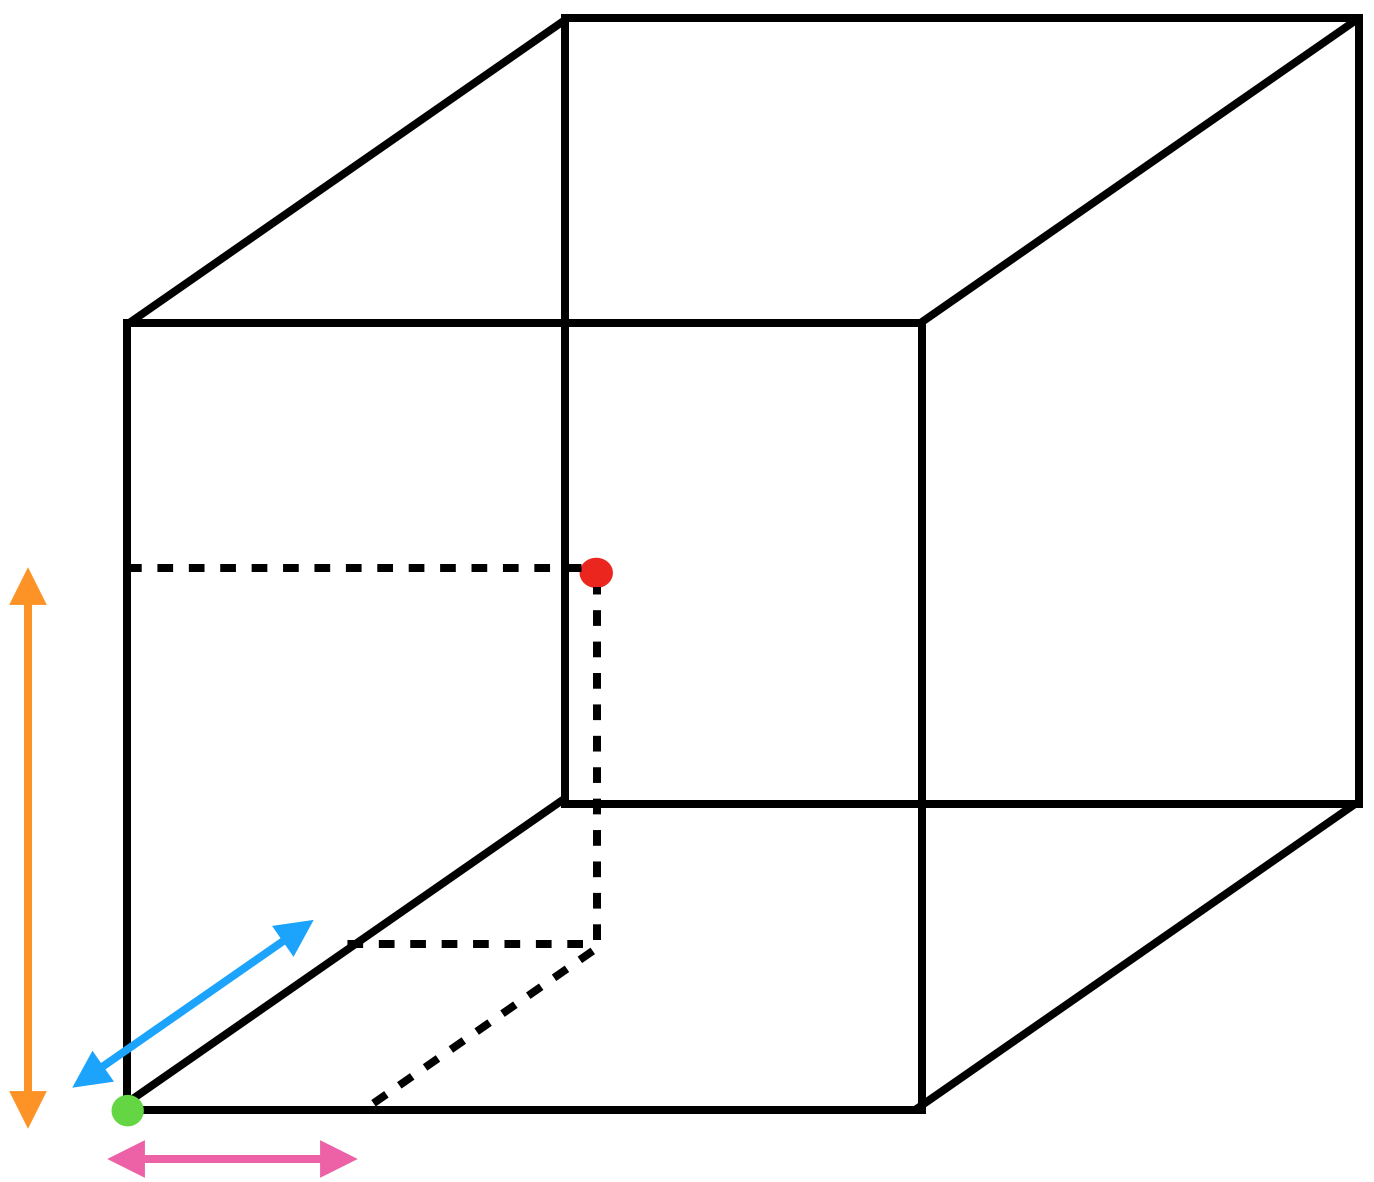
\includegraphics[scale=0.3]{cube}
\caption{Visualisation of a cube surrounding a particle, where the vertices of the cube represent the grid points of the density mesh.}
\label{cube}
\end{figure}
The particle in this figure is deliberately not placed at the center of the cube to show that each grid point (vertice) gets a different amount of fraction of the mass of the particle. The green grid point is second closest to the particle (the closest is the grid point just above this one). Using interpolation, the mass it gets assigned to is now the size of the pink arrow times the size of the blue arrow times the size of the orange arrow. Using this logic, it can be seen that the grid point opposite the green one (which is furthest away from the particle) gets less mass of the particle. So to summarize, the mass of the particle is split up in 8 bits. Each bit is determined by how close the particle is to the grid point. The code that is used to create this algorithm, including the robustness check, is shown below,

\lstinputlisting[firstline = 77, lastline = 163]{Q5.py}

The output of the code are again 4 plots of the $x - y$ grid for $z = 4,9,11,14$, together with the same robustness check plot as shown in the previous section.

\begin{figure}[h]
\centering
\includegraphics[scale=0.9]{plots/CIC_9.png}
\caption{Mass assignment scheme for $z = 4$ (left figure) and $z = 9$ (right figure).}
\label{cic1}
\end{figure}

\begin{figure}[h]
\centering
\includegraphics[scale=0.9]{plots/CIC_14.png}
\caption{Mass assignment scheme for $z = 11$ (left figure) and $z = 14$ (right figure).}
\label{cic2}
\end{figure}

\begin{figure}[h]
\centering
\includegraphics[scale=0.6]{plots/CIC_test.png}
\caption{The fraction of the mass of the particle assigned to the cell plotted against the position of the particles. The orange line is for cell 0 and the blue line if for cell 4.}
\label{cic_test}
\end{figure}

The white spots represent again cells which do not have mass assigned to it at all. The amount of white patches is, however, less in these 4 figures than the amount of white patches in the 4 figures shown in section 5.1. In addition, the patches that show mass seem to overflow a tiny bit from one to another (i.e. there seems to be some smoothness in the figures). Looking at figure \ref{cic_test}, one can see that this method is less discrete than the NGP method. The amount of mass assigned to the cells one and four increases as it approaches the grid point and decreases again when it moves away from the grid point. Just as expected what should happen when using interpolation.
\clearpage

\subsection{Fast Fourier Transform}

A method for computing the fourier transform numerically is the fast fourier transform. To be more specific, the method that is going to be discussed in this section is the Cooley-Tukey FFT. The fast fourier transform makes use of the fact that the fourier transform is symmetric. The discrete fourier transform is given by,

\begin{equation*}
X_k = \sum_{n=0}^{N-1}x_n e^{-\frac{2\pi i}{N}nk}
\end{equation*}
where $k$ is an integer that is ranging from 0 to $N-1$. Here $N$ is the number of data points. The simplest Cooley-Tukey algorithm splits the function $x_n$ into two parts. It is split into a sum over the even indices, and a sum over the odd indices,
\begin{equation*}
X_k = \sum_{m=0}^{\frac{N}{2} - 1} x_{2m}e^{-\frac{2\pi i}{N}(2m)k} + \sum_{m=0}^{\frac{N}{2}-1}x_{2m+1}e^{-\frac{2\pi i}{N}(2m+1)k}
\end{equation*}
In the second sum, it is possible to factor the term $e^{-\frac{2\pi i}{N}k}$ out. So now we get,
\begin{equation*}
X_k = \sum_{m=0}^{\frac{N}{2}-1}x_{2m}e^{-\frac{2\pi i}{N/2}mk} + e^{-\frac{2\pi i}{N}k}\sum_{m=0}^{\frac{N}{2}-1}x_{2m+1}e^{-\frac{2\pi i}{N/2}mk}
\end{equation*}
Now due to symmetry we have that $X_{k + \frac{N}{2}}$ can also be obtained with the odd and even parts of $x_n$,
\begin{gather*}
X_{k+\frac{N}{2}} = \sum_{m=0}^{\frac{N}{2}-1}x_{2m}e^{\frac{-2\pi i}{N/2}m(k+\frac{N}{2})} + \sum_{m=0}^{\frac{N}{2}-1} x_{2m+1}e^{-\frac{2\pi i}{N}(2m+1)(k+\frac{N}{2})}\\
=  \sum_{m=0}^{\frac{N}{2}-1}x_{2m}e^{\frac{-2\pi i}{N/2}m(k+\frac{N}{2})}\cdot e^{-2\pi m i} + e^{-\frac{2\pi i}{N}(k + \frac{N}{2})}\sum_{m=0}^{\frac{N}{2}-1} x_{2m+1} e^{-\frac{2\pi i}{N/2}m(k+\frac{N}{2})}\\
= \sum_{m=0}^{\frac{N}{2}-1}x_{2m}e^{\frac{-2\pi i}{N/2}m(k+\frac{N}{2})}\cdot e^{-2\pi m i} + e^{\frac{2\pi i}{N}k}e^{-\pi i}\sum_{m=0}^{\frac{N}{2}-1} x_{2m+1} e^{-\frac{2\pi i}{N/2}m(k+\frac{N}{2})}
\end{gather*}
The terms $e^{2\pi m i}$ and $e^{\pi i}$ are 1 and minus 1 respectively, and therefore the equation above becomes,
\begin{equation*}
X_{k+\frac{N}{2}} =  \sum_{m=0}^{\frac{N}{2}-1}x_{2m}e^{\frac{-2\pi i}{N/2}m(k+\frac{N}{2})} - e^{\frac{2\pi i}{N}k}\sum_{m=0}^{\frac{N}{2}-1} x_{2m+1} e^{-\frac{2\pi i}{N/2}m(k+\frac{N}{2})}
\end{equation*}
Using this symmetry makes computing the fourier transform much more efficient. Using these equations recursively makes this fast fourier transform extremely efficient. There is, however, another way to compute it with the use of bit-reversal. This is known as another variant of the Cooley-Tukey algorithm but is not used in this solution paper. The code that has been used to compute this is shown below,

\lstinputlisting[firstline = 165, lastline = 216]{Q5.py}
The output of this code is the fourier transform of the function $\cos(40\pi x)$ gotten from the own implementation, the one from scipy and the analytical solution.

\begin{figure}[h]
\centering
\includegraphics[scale=0.6]{plots/FFT_1D.png}
\caption{The fourier transform of $\cos(40\pi x)$, where the blue dotted line is the solution from scipy, the orange line is the own implementation and the red lines is the analytical solution}
\label{FFT_1D}
\end{figure}

It can be seen from the figure \ref{FFT_1D} that the scipy solution and the own implementation are exactly the same. The analytical solution is obtained by noticing that the fourier transform of this particular function is simply a delta function,

\begin{equation*}
\mathrm{FT} \propto \delta\left(\omega - 40\pi\right) + \delta\left(\omega + 40\pi\right) 
\end{equation*}
where $\omega$ are the frequencies. This delta function is of course analytically simply a vertical line. However, because we have a discrete function, it is not possible to create a vertical line that goes to infinity, and therefore a small dispersion will be seen in the graph. The positions of the peaks are at the exact same spot, which is as expected. Note that there are two peaks, this is because in fourier space we have negative and positive frequencies.

\subsection{Fast Fourier Transform in 2D and 3D}

Now that we've shown that the 1D fourier transform seems to work fine, it is also possible to do this in 2 and 3 dimensions. This can be done by simply fourier transforming over each dimension. So for the 2D FFT this would be transforming the rows and columns separately, and for the 3D FFT this would be transforming the arrays in the x, y, and z axis separately. The code that is used for this is shown below,

\lstinputlisting[firstline = 218, lastline = 354]{Q5.py}
The output of the code is for the 2D fft the fourier transform of the function $\cos(0.2\pi(X+Y))$, where $X$ and $Y$ are 2D matrices, with the use of the own implementation and the one from scipy. I did not manage to convert the axes of this 2D plot to the right frequencies, and therefore I also did not manage to plot the analytical version. The analytical version would resemble a delta function again, but now in 2D. It would peak at $\omega_x = \omega_y = 0.2\pi$ and $\omega_x = \omega_y = -0.2\pi$. For the 3D plot, the multivariate gaussian has been fourier transformed, using the own implementation and the own from scipy. This 3D matrix has been sliced to get the x-y, y-z, and x-z grids at the center of the matrix.
\begin{figure}[h]
\centering
\includegraphics[scale=0.5]{plots/real_space_2D.png}
\caption{The real-spaced function $\cos(0.2\pi(X+Y))$.}
\end{figure}
\begin{figure}[h]
\centering
\includegraphics[scale=0.8]{plots/FFT_2D.png}
\caption{The fourier transform of the 2D function. Left: scipy fourier transform, right: own implementation}
\end{figure}
\begin{figure}[h]
\centering
\includegraphics[scale=0.85]{plots/gauss_XY.png}
\caption{The fourier transform of the 3D function. Left: scipy fourier transform, right: own implementation. This figure represents the $x-y$ grid.}
\end{figure}
\begin{figure}[h]
\centering
\includegraphics[scale=0.85]{plots/gauss_YZ.png}
\caption{The fourier transform of the 3D function. Left: scipy fourier transform, right: own implementation. This figure represents the $y-z$ grid.}
\end{figure}
\begin{figure}[h]
\centering
\includegraphics[scale=0.85]{plots/gauss_XZ.png}
\caption{The fourier transform of the 3D function. Left: scipy fourier transform, right: own implementation. This figure represents the $x-z$ grid.}
\end{figure}

Both the figures of the 2D fourier transform and the 3D fourier transform seem to match the scipy implementation quite well. The 2D fourier transform should have been two scatter points without any dispersion. However, as mentioned in the previous section, numerically this can not be computed since the delta function is not defined numerically. We can see also that the amplitudes of these yellow dots are extremely high which indicates that this delta function is done relatively well. We'd expect these amplitudes to go to infinity but, of course, this is numerically not possible. The analytical solution would match this one quite well, though it would not have these dispersion lines seen in the x and y directions. 
\clearpage

\section{Classifying $\gamma$-ray bursts}

Logistic regression is a way to classify data given some already labelled data. In this exercise, long $\gamma$-ray bursts are classified according to their certain characteristics other than time it has been observed. $\gamma$ ray bursts are classified as short or long based on their time scale. If the burst has been received for over 10 seconds, then it is identified as a long $\gamma$ ray burst. The dataset that was given contains multiple gamma ray bursts where the time within which the detector receives $90\%$ of the $\gamma$-rays is given. In addition, some other properties of the host galaxy were given, such as the redshift. In this exercise, logistic regression is used to determine whether we deal with a long or short GRB (Gamma Ray Burst) depending on some of the characteristics of the host galaxy. The data given contains a lot of missing data. To correct for this, we first set all the missing data (data elements that have value -1) to 0. However, two columns are in log-space. The exponent of these elements in these columns are first taken. All the data that now corresponds to $\exp(-1)$ is set to 0. The final two columns are not considered in the train set because these contain too many missing data elements. In the first column there were some names that did not correspond to the GRB name (XRF). Just to be sure not to use data that is not representative, these rows were taken out of the train data. The labels are created by looping over the some rows but now for the third column that contains the time within which the detector receives $90\%$ of the $\gamma$-rays, $T_{90}$. If it is higher or equal to 10, then the label is set to 1, otherwise it is set to 0. Now that the data is complete, logistic regression is used to predict the labels with the use of the given characteristics.\footnote{Since this was the last exercise that I had to do, I unfortunately have no time left to explain exactly how logistic regression works.} The code that is used for this question is shown below,

\lstinputlisting{Q6.py}
The output of the code is a histogram that contains the predicted labels and the actual labels. 

\begin{figure}[h]
\centering
\includegraphics[scale=0.6]{plots/logistic_regression.png}
\caption{A histogram of the predicted labels (orange) vs. the actual labels (blue), where the predicted labels were obtained with the use of logisitc regression.}
\end{figure}

The histograms show that the logistic has done an adequate job, although it has still mislabelled quite some data. The accuracy that was obtained was $80\%$. However, there were some strange things happening while running the program. First of all, the number of epochs that have been used was only 2, which is quite unlikely if the logistic regression had done a good job. The reason for this is because many of the predicted labels were straight away set to 1. In the loss function this will go wrong since $\log(0)$ is not defined. Therefore, an extra term of 0.0001 was added to make sure that no nans were returned in this part of the run. This is not a nice way to do it, however, I just didn't manage to get it work otherwise. It could be that I have made a small mistake in the code where I add/multiply in the wrong way. Unfortunately, I could not find this mistake. Another explanation could be that I did not prepare my data well enough. A solution for this in the future would be to first check if I expect some correlation between columns beforehand before selecting the data. All in all, the logistic regression that I used did manage to overpass the baseline of $77.8\%$.\footnote{Sice $77.8\%$ of the data is equal to a long, setting all the predicted labels to long would result in an accuracy of $77.8\%$.} The question remains where in the algorithm it goes wrong.

\section{Building a quadtree}

The Barnes-Hut quadtree has many uses in the astrophysics. One key idea of such a tree is to calculate the combined effect of group particles together. In this exercise, this is done by calculating the multipole moments of first order $n=0$. The multipole moment of $n^{\mathrm{th}}$ order is given by,

\begin{equation*}
M_n (z_a) = \sum_{a} m_a \frac{1}{n!}(x_a - z_A)^{n!}
\end{equation*}

where $z_A$ is the centre of the group particles, $n$ is the moment to be calculated,
$x_a$ is a particle within the group of particles, and $m_a$ are the belonging masses of each particle. For the first order multipole moment, $n=0$, this expression reduces to,
\begin{equation*}
M_0 = \sum_a m_a
\end{equation*}
Here it is assumed that $z_A$ is the centre of mass of the group. Thus,
 it is the sum of masses of all particles within the group. Using a quadtree, groups of particles can be formed and the multipole moment of each group can then be calculated for $n=0$. For this quadtree, a maximum of 12 particles were contained in each leaf. If a node contains more than 12 particles, it divides itself up in 4 new nodes. These 4 new nodes are also known as the 'north-west', 'south-west', 'north-east', and 'south-east' nodes, since these are the directions where the new nodes end up. For each node in the tree, the multipole moment can be calculated by summing the masses of all the particles contained in the node. The dataset that has been given to us contains the x-y positions of 1200 particles together with the mass of each particle. However, I have checked the data beforehand and noticed that the mass of each particle is exactly the same. Ignoring the units, each particle has mass $0.012500000186264515$. So instead of using each mass in the tree, the multipole moments are calculated by summing the amount of particles within a node and then multiplying it by this given mass. The code that produces such a tree is shown in below,
 \lstinputlisting{Q7.py}
 
 The output of the code is a plot of the tree where the particles are scatter plotted and each node is plotted over this scatter plot as a rectangle. In addition, the multipole moment for the leaf node containing the particle with index $i = 100$ and all of its parent nodes (including the root node) has been saved in a textfile.
 
 \lstinputlisting{textfiles/tree.txt}
 
 \begin{figure}[h]
 \centering
\includegraphics[scale=0.7]{plots/tree.png} 
 \caption{The quad tree containing all particles and all nodes and leafs. The nodes and leafs are indicated by the squares.}
 \label{Tree}
 \end{figure}

It can be seen from figure \ref{Tree} that the positions of the particles are quite clustered. Nevertheless the tree does seem to do a good job in assigning all the particles to the correct node. It can also be seen that the multipole moments seem to be correct at least the for the first node (the complete tree) and for the leaf. For the first node we'd expect a multipole moment of $1200\cdot0.012500000186264515 = 15.000000223517418$, which is exactly what the textfile also reads. For the leaf we'd expect a maximum multipole moment of $12\cdot 0.012500000186264515  = 0.15000000223517418$. The multipole moment the tree found in this leaf was $\sim 0.125$, which is smaller than the maximum, and thus it could certainly be the correct answer. All in all, the tree has successfully been build.

\clearpage

%\input{8}

\end{document}
